\subsection{The Standard Model of particle physics}

\begin{frame}{The Standard Model (SM) of particle physics}

\begin{columns}
\column{0.5\textwidth}

\begin{itemize}
    \item Quantum field theory, based on the principal gauge invariance $\textcolor{HHturquoise_d}{SU(3)}\times \textcolor{HHturquoise_l}{SU(2)}\times \textcolor{HHturquoise_l}{U(1)}$
    \item Unify \textbf{\textcolor{HHturquoise_d}{Strong}} and \textbf{\textcolor{HHturquoise_l}{Electro-weak}} interactions.
    \item Fermions: matter particles
    \begin{itemize}
        \item \textcolor{violet}{Quarks}
        \item \textcolor{applegreen}{Leptons}
    \end{itemize}
    \item \textcolor{cadmiumorange}{Gauge bosons}: mediators of interactions
\end{itemize}    
\begin{itemize}    
    \item \textcolor{HHyellow}{Higgs boson}
    \begin{itemize}
        \item Responsible for mass generation through EWSB mechanism
    \end{itemize}
\end{itemize}

\column{0.5\textwidth}
\begin{figure}
    \centering
    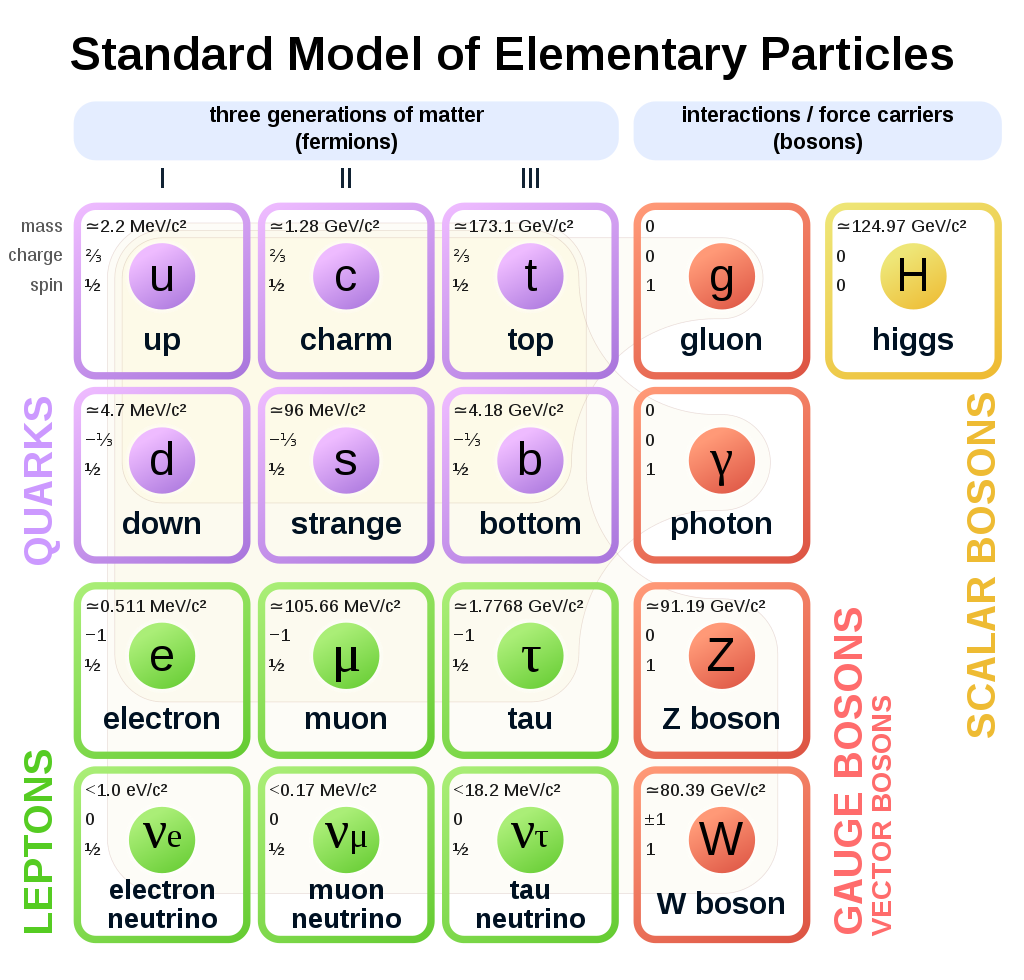
\includegraphics[width=1\textwidth]{Part1/Img/SM_particles.png}
\end{figure}
\end{columns}
\end{frame}

\begin{frame}{Electroweak Symmetry Breaking and Higgs boson}
\setbeamercovered{transparent}
\begin{columns}
\column{0.4\textwidth}
\begin{figure}
    \centering
    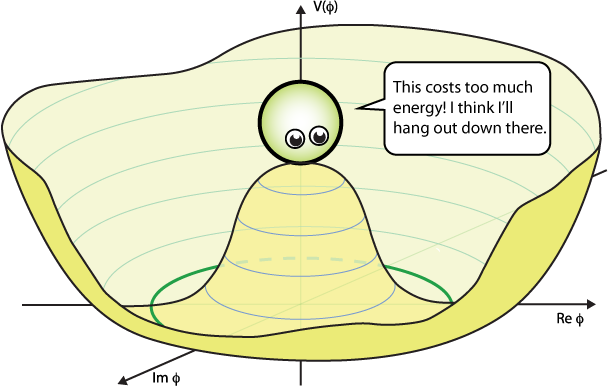
\includegraphics[width=0.8\textwidth]{Part1/Img/Higgs-Potential-lookdown.png}
\end{figure}
\visible<2>{
\begin{figure}
    \centering
    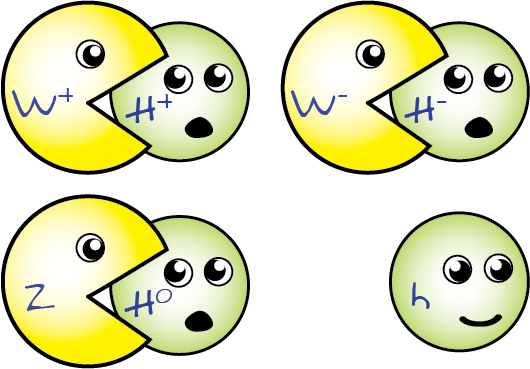
\includegraphics[width=0.8\textwidth]{Part1/Img/Goldstone-Eaten-four.png}
\end{figure}
}
\column{0.6\textwidth}
gauge boson mass terms break gauge symmetry of SM:
\begin{itemize}
    \item \textcolor{structurColor}{Brout-Englert-Higgs (1964)} include complex scalar field:
    \begin{equation*}
        V(\phi^\dagger\phi) = \mu^2\phi^\dagger\phi + \lambda(\phi^\dagger\phi)^2
    \end{equation*}
    \pause
    \item Choice of the vacuum state \textbf{\textcolor{applegreen}{spontaneously breaks the symmetry}}:
    \begin{itemize}
        \item Gauge bosons become massive
        \item Higgs boson: weakly constrained mass
        \item Fermion masses: generated through Yukawa couplings
    \end{itemize}
\end{itemize}

\begin{itemize}
    \item \underline{Observed} in 2012 at LHC, $m_{H} \sim $ 125 GeV
\end{itemize}
\end{columns}
\end{frame}

\begin{frame}{Measurements of Higgs parameters}

\begin{figure}
    \centering
      \subfloat{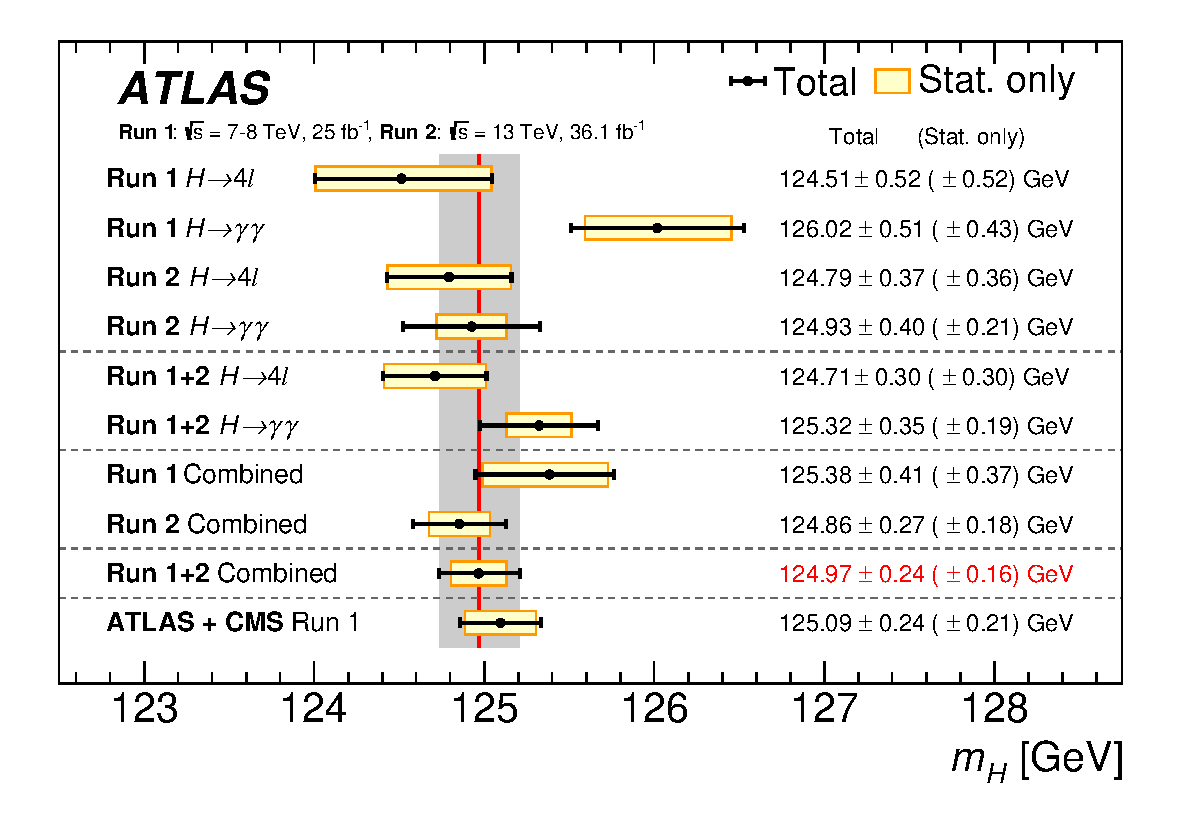
\includegraphics[width=0.35\textwidth]{Part1/Img/ATLAS_HIGGS1100_mass_Summary.pdf}}
      \subfloat{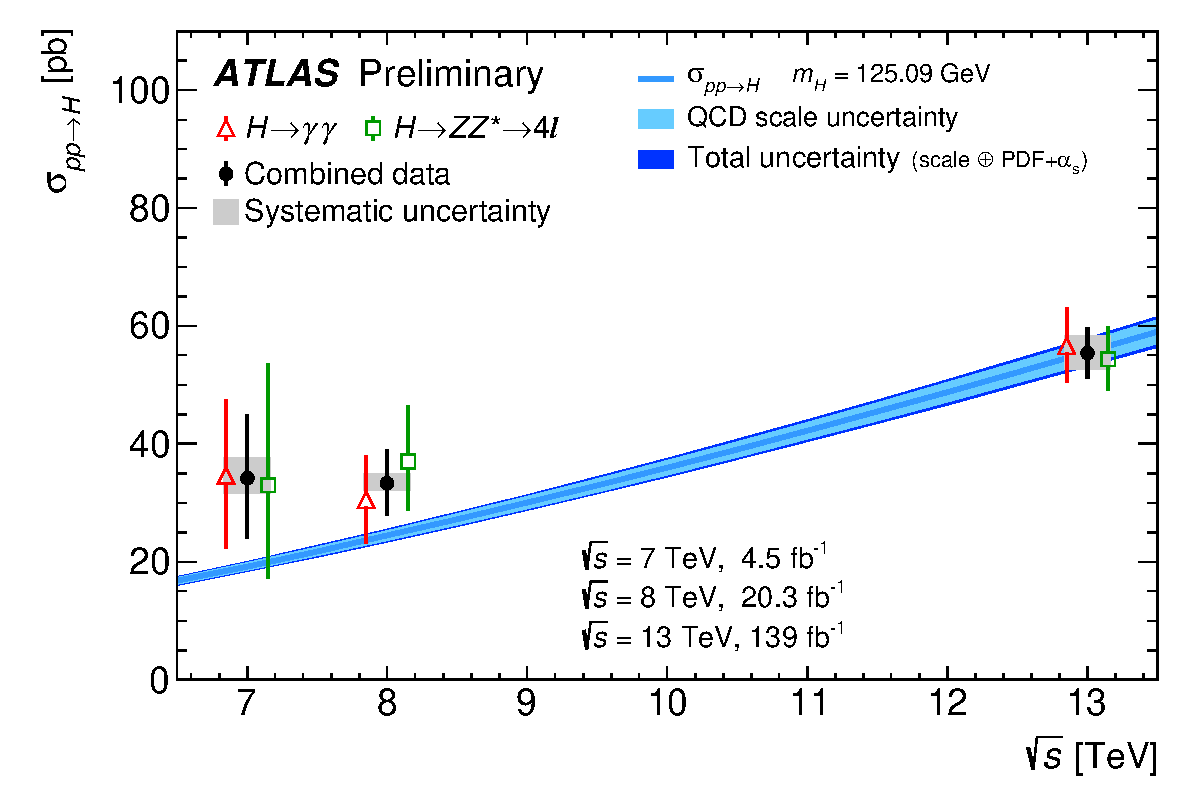
\includegraphics[width=0.35\textwidth]{Part1/Img/ATLAS_HIGGS3010_XSvsCME_Summary.pdf}}
%    \subfloat{ 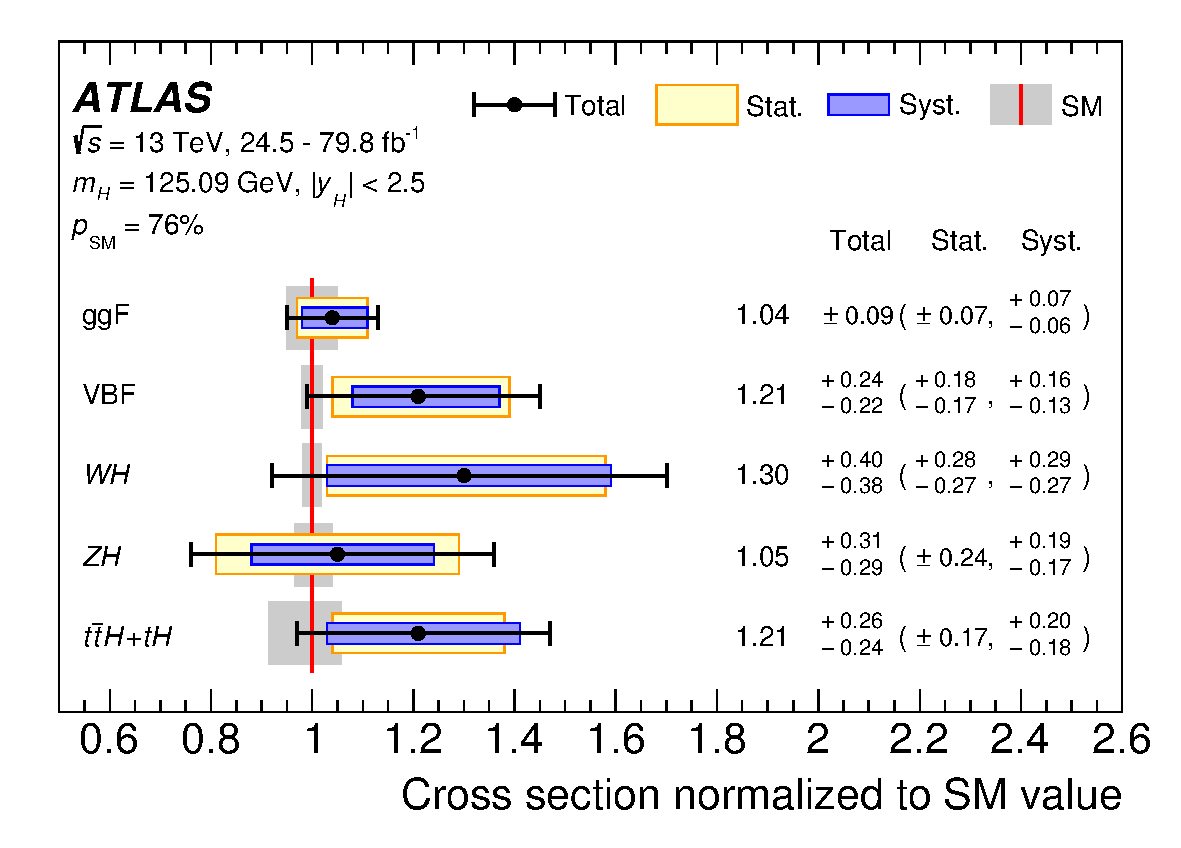
\includegraphics[width=0.5\textwidth]{Part1/Img/ATLAS_HIGGS3250_Run2XS_Summary.pdf}}
      \subfloat{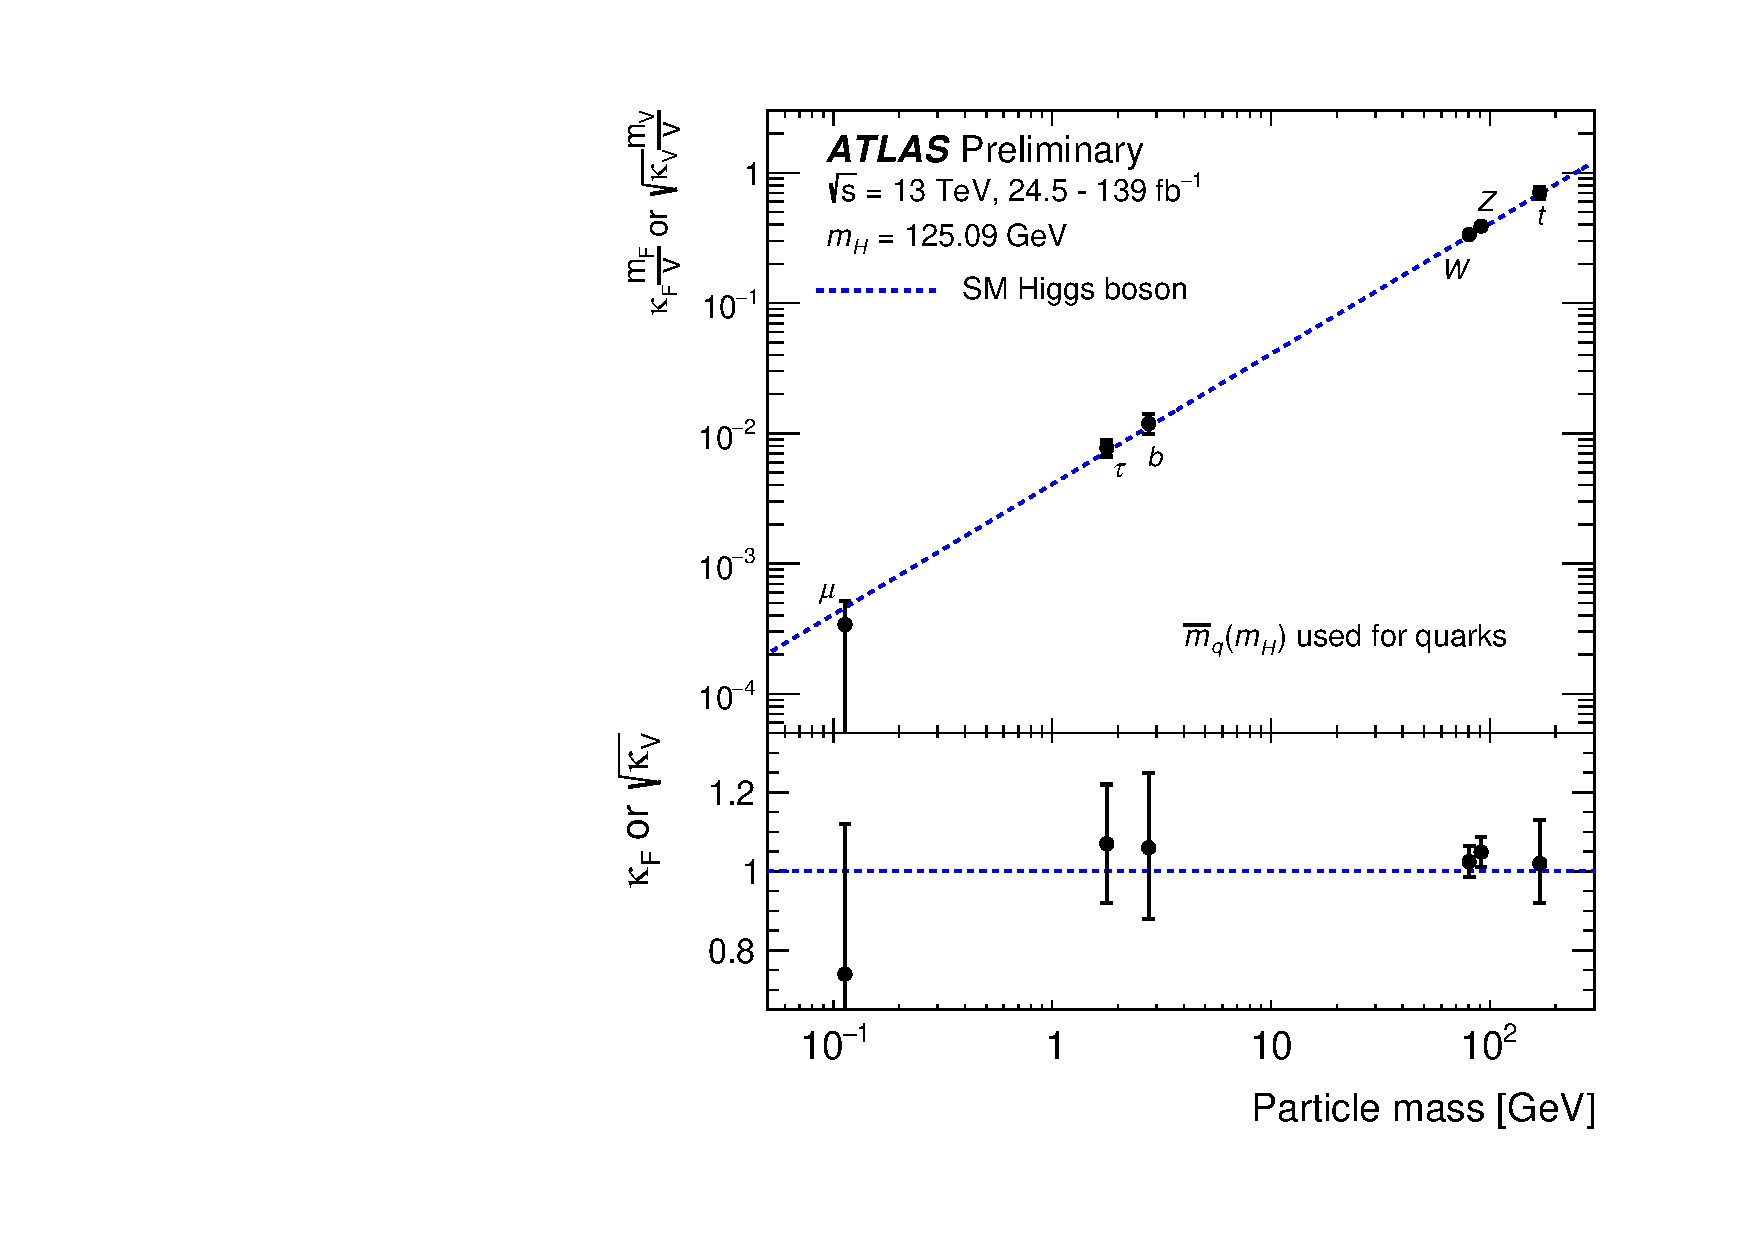
\includegraphics[width=0.35\textwidth]{Part1/Img/ATLAS_HIGGS4400_kappa_vs_mass.pdf}}
\end{figure}

\begin{itemize}
    %\item Mostly measured:
    %\begin{itemize}
    %    \item \textcolor{HHturquoise_l}{mass}
    %    \item \textcolor{HHturquoise_m}{cross-section}
    %    \item \textcolor{HHturquoise_d}{coupling to bosons and fermions}
    %\end{itemize}
    \onslide<2>{
    \item \textcolor{HHred}{Not all, Higgs boson self-coupling still resists to physicists}
    }
\end{itemize}

\end{frame}

\subsection{Higgs boson self-coupling}

\begin{frame}{Higgs boson self-coupling}
\begin{columns}
\column{0.6\textwidth}    
\begin{itemize}
    \item \textbf{\textcolor{structurColor}{Higgs boson trilinear coupling} : self-coupling}
    \item Controls the shape of the Higgs potential
    \item Physics beyond SM (BSM) physics can impact this shape
    \item BSM impact quantified as:
    \begin{equation*}
       \textcolor{HHred}{\kappa_{\lambda} = \frac{\lambda}{\lambda^{SM}}}
    \end{equation*}
     \item Motivation to experimentally reconstruct Higgs potential shape
    \onslide<3>{
    \item measured \underline{\textbf{directly}} with \textbf{\textcolor{HHturquoise_d}{Higgs boson pair (\textbf{HH}) production}} 
    \item not observed yet $\to$ limit on production cross-section
    }
\end{itemize}

\column{0.4\textwidth}  
\begin{equation*}
    V \supset \lambda v^2H^2 + \textcolor{HHred}{\lambda vH^3} + \frac{\lambda}{v}H^4
\end{equation*}
\begin{equation*}
    \lambda = \frac{m_{H}^2}{2v^2}
\end{equation*}
\begin{center}
$\lambda^{SM} \sim 0.13$   
\end{center}
\begin{figure}
    \begin{overprint}
    \onslide<1>\centering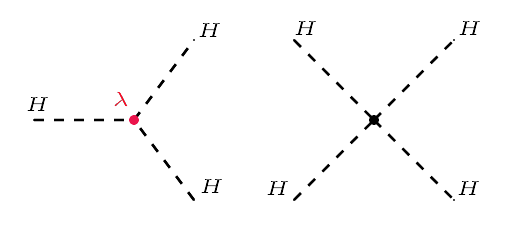
\includegraphics[width=0.9\textwidth]{Part1/Img/hhh_diagrams.png}
    \onslide<2>\centering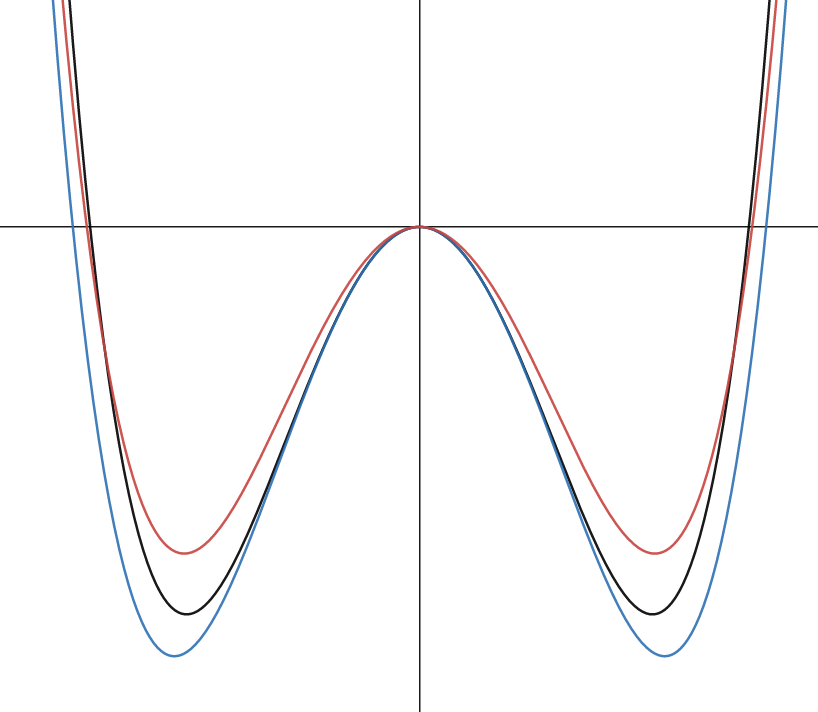
\includegraphics[width=0.8\textwidth]{Part1/Img/schematic_Higgs_potential.png}
    \onslide<3>\centering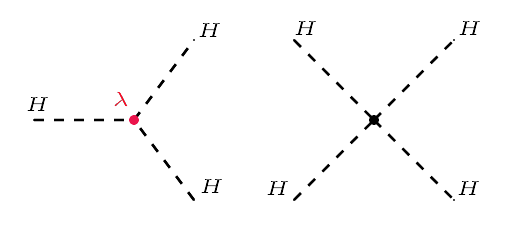
\includegraphics[width=0.9\textwidth]{Part1/Img/hhh_diagrams.png}
    \end{overprint}
\end{figure}

\end{columns}    

\end{frame}

\subsection{Higgs boson pair production}

\begin{frame}{Higgs boson pair production at the LHC}

\begin{itemize}
    \item At the LHC, mainly produced via \textbf{\underline{non-resonant}} \textbf{\textcolor{HHred}{ggF}} and \textbf{\textcolor{HHturquoise_d}{VBF}} modes. 
\end{itemize}

\begin{figure}
    \fcolorbox{HHred}{HHwhite2}{     \subfloat{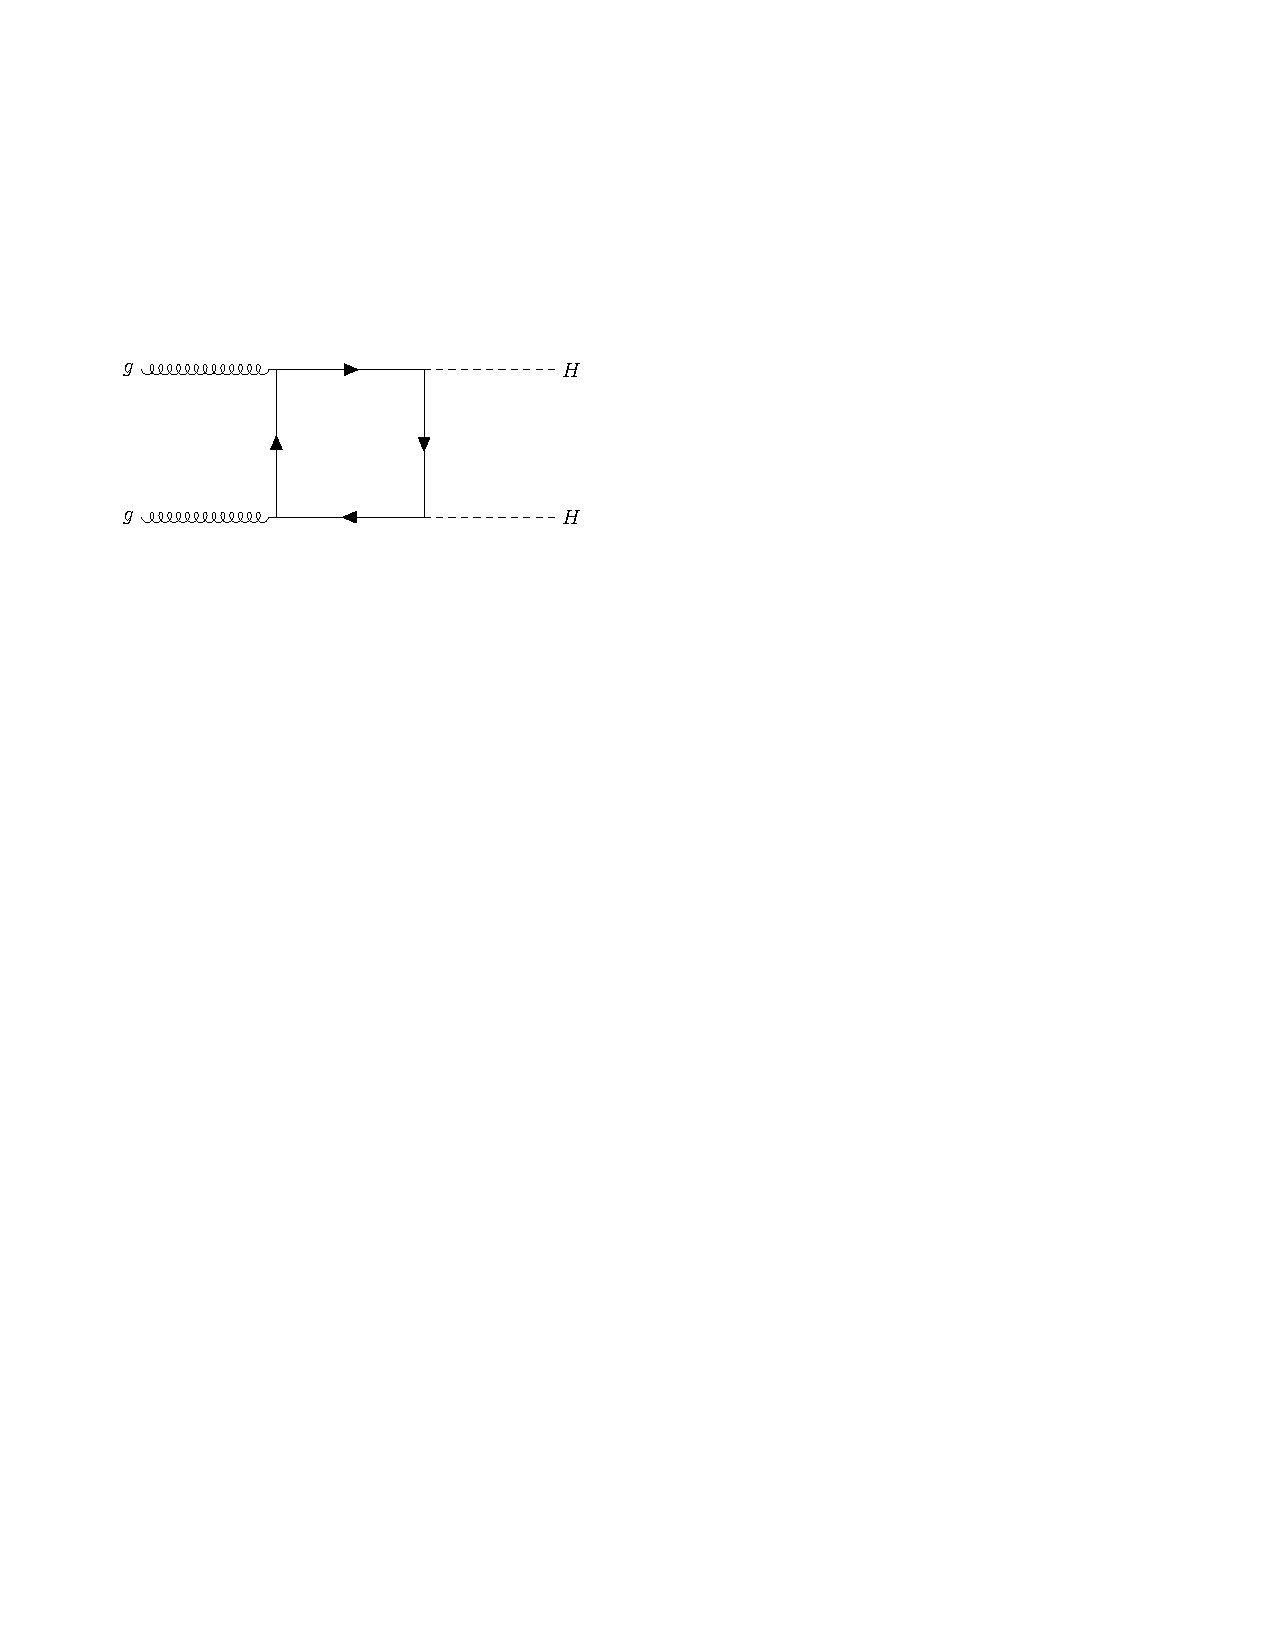
\includegraphics[width=0.25\textwidth]{Part1/Img/ggF_box.pdf}}
    \subfloat{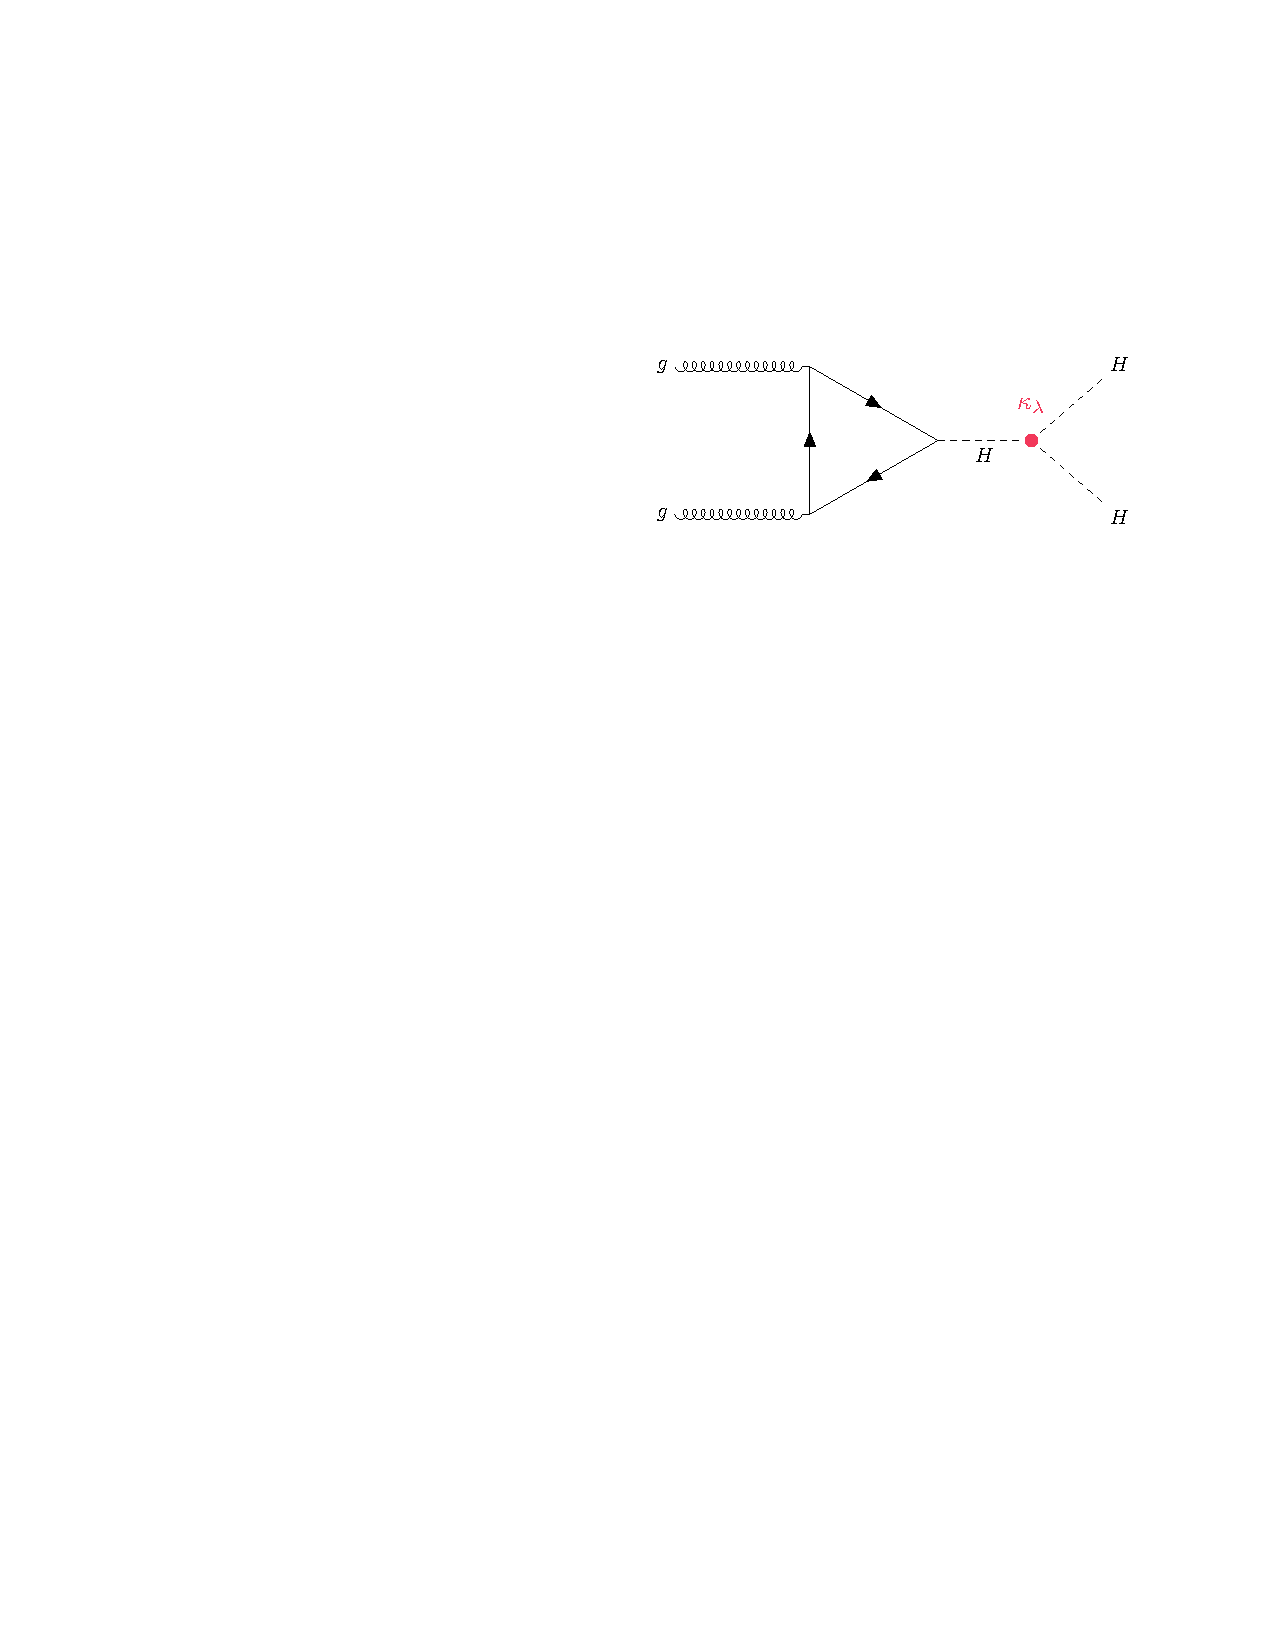
\includegraphics[width=0.25\textwidth]{Part1/Img/ggF_tri.pdf}}}
    \fcolorbox{HHturquoise_d}{HHwhite2}{
    \subfloat{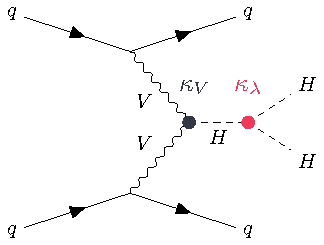
\includegraphics[width=0.17\textwidth]{Part1/Img/VBF_kvkl.pdf}}
    }
\end{figure}




\begin{itemize}
    \item At 13 TeV, $m_{H} = $ 125.09 GeV and $\kappa_{\lambda} = $ 1: 
    \begin{itemize}
        \item \textcolor{HHred}{\textbf{$\sigma^{ggF}_{HH} = $ 31.05 fb}}, 1000$\times$ smaller than $\sigma_{H}$
        \item \textcolor{HHturquoise_d}{\textbf{$\sigma^{VBF}_{HH} = $ 1.73 fb}}, one order of magnitude smaller than ggF
    \end{itemize}
\end{itemize}

\end{frame}

\begin{frame}{Di-Higgs boson as a probe of BSM physics}

\begin{columns}
\column{0.6\textwidth} 
\begin{itemize}
    \item Challenging low cross-section, BSM anomaly may enhance it
    \item BSM physics can manifest as deviation:
    \begin{itemize}
        \item \textbf{\textcolor{HHred}{Total}} cross-section
        \item \textbf{\textcolor{HHturquoise_m}{Differential}} cross-section
    \end{itemize}
    \item Measurement of $\kappa_{\lambda}$ may indicate presence of BSM physics 
\end{itemize}
%\onslide<2>{
%\underline{Thesis aim}: \textbf{search for HH events in the $b \bar{b}\gamma\gamma$ final state and constrain $\kappa_{\lambda}$}
%}
\column{0.4\textwidth}  

%\begin{figure}
%    \centering
%    \fcolorbox{HHred}{HHwhite2}{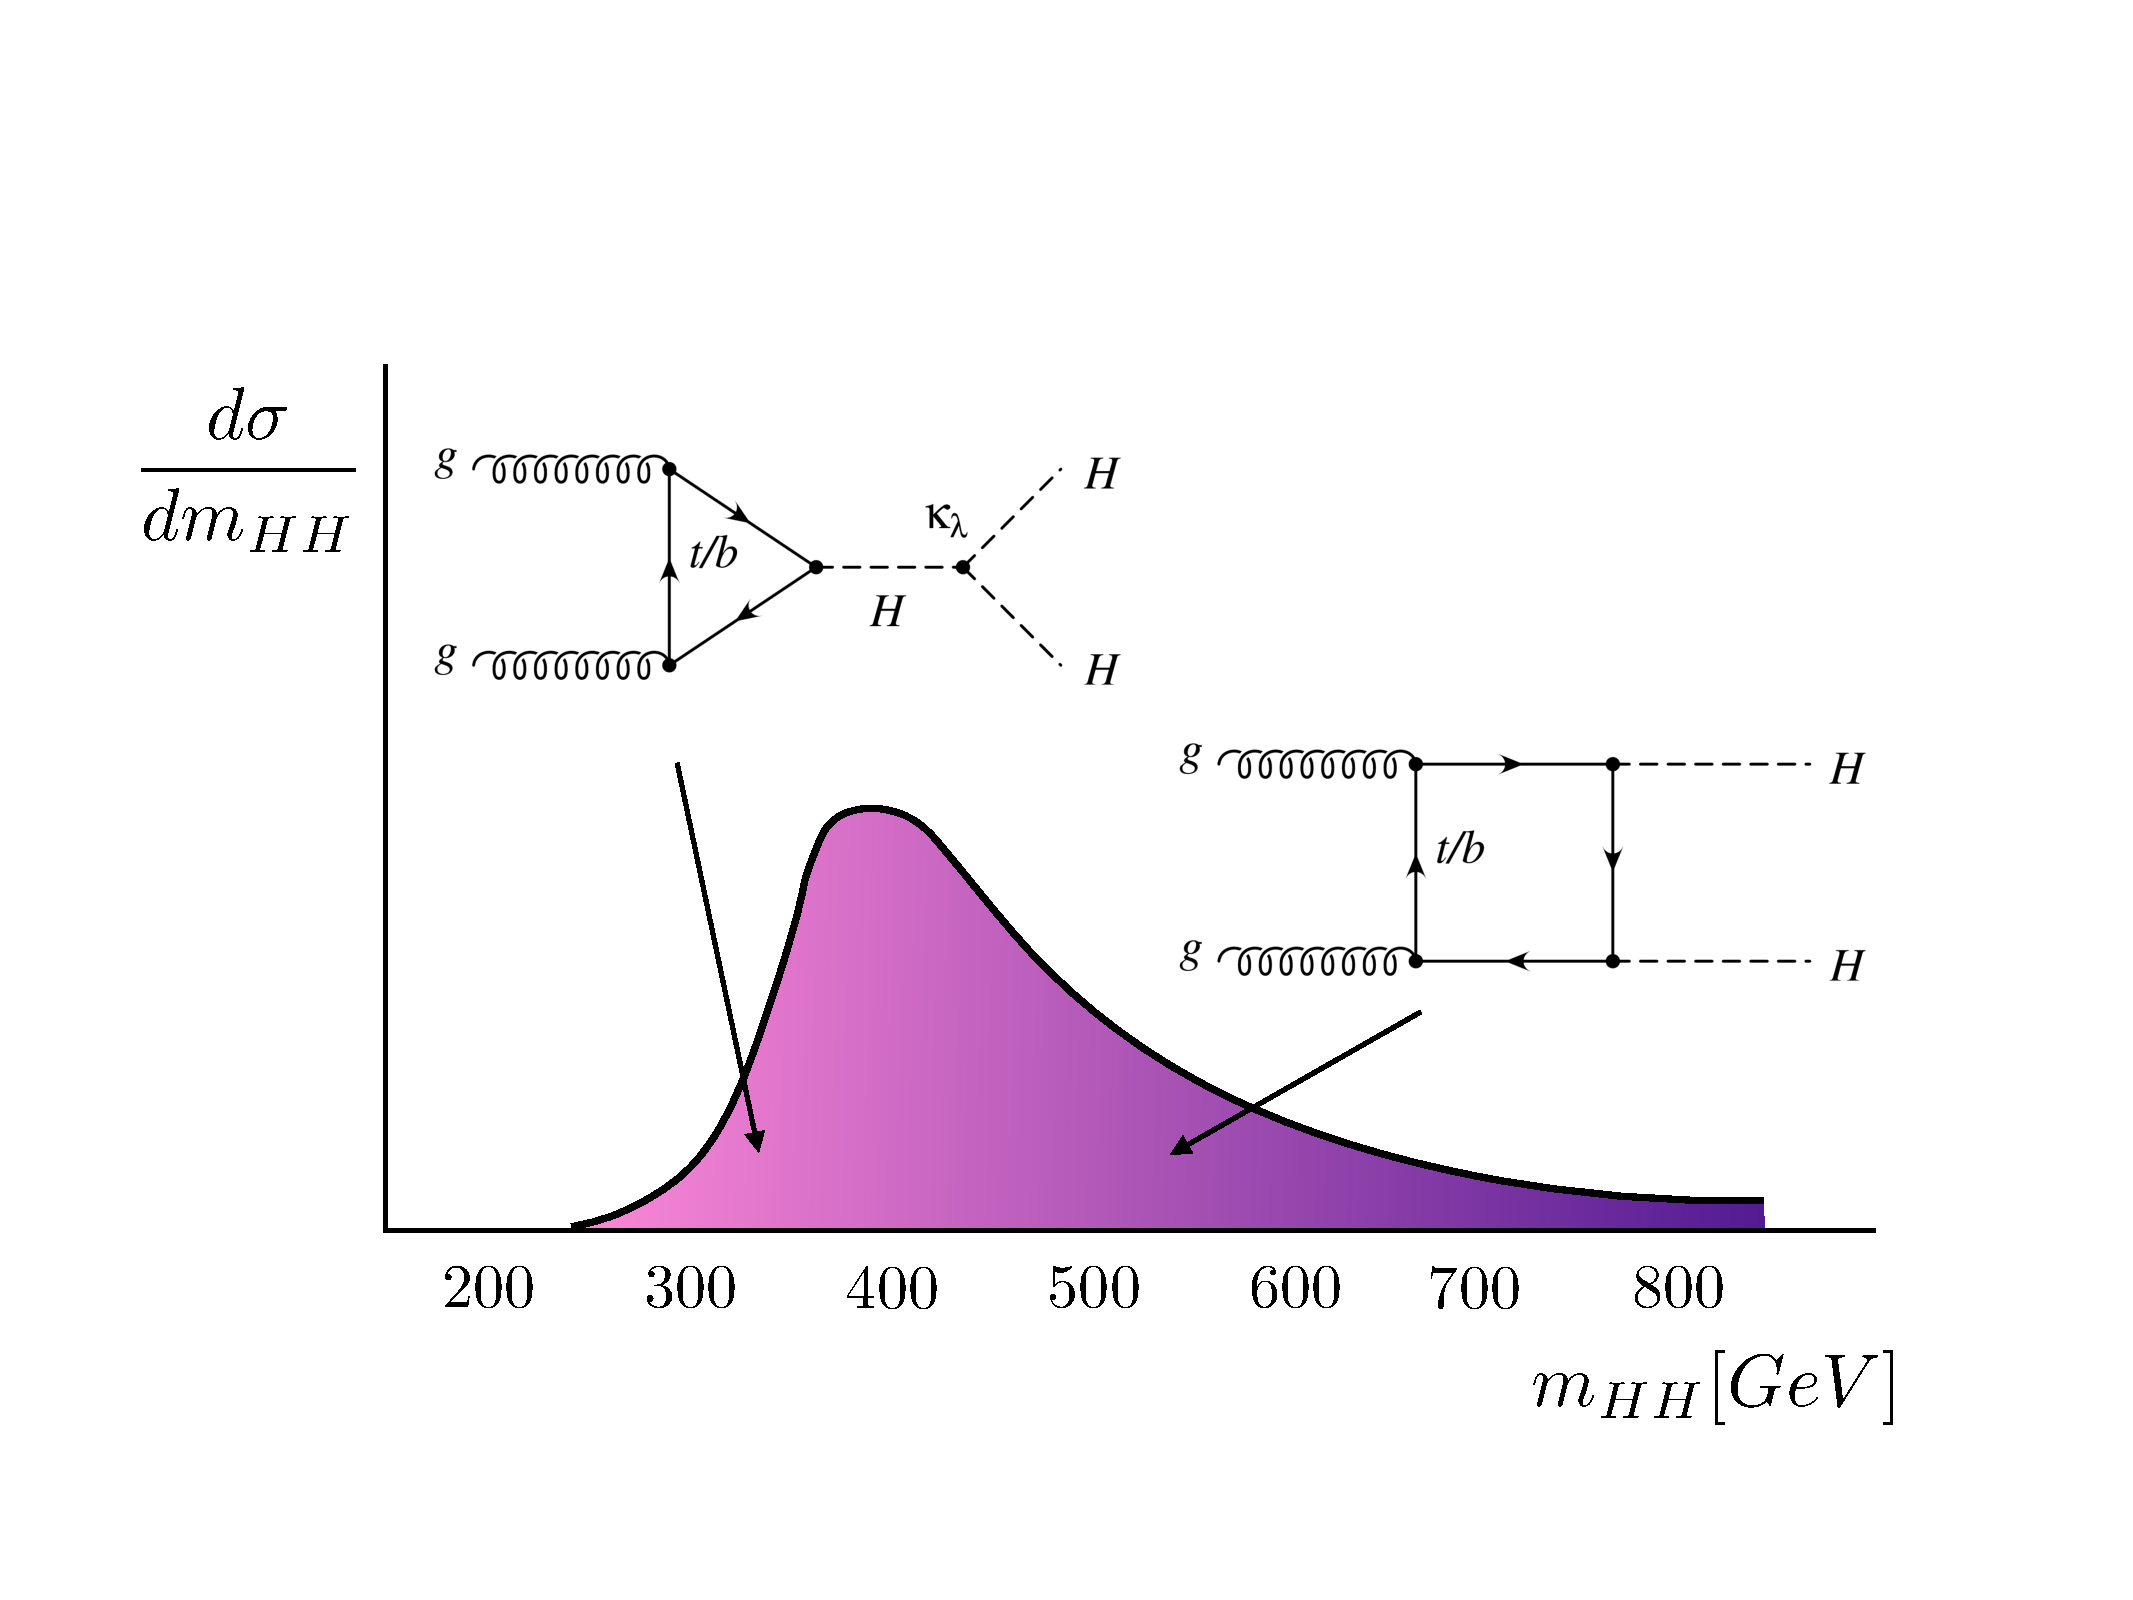
\includegraphics[width=0.7\textwidth]{Part1/Img/mHHSketch.pdf}}
%\end{figure}

\begin{figure}
    \centering
    \fcolorbox{HHred}{HHwhite2}{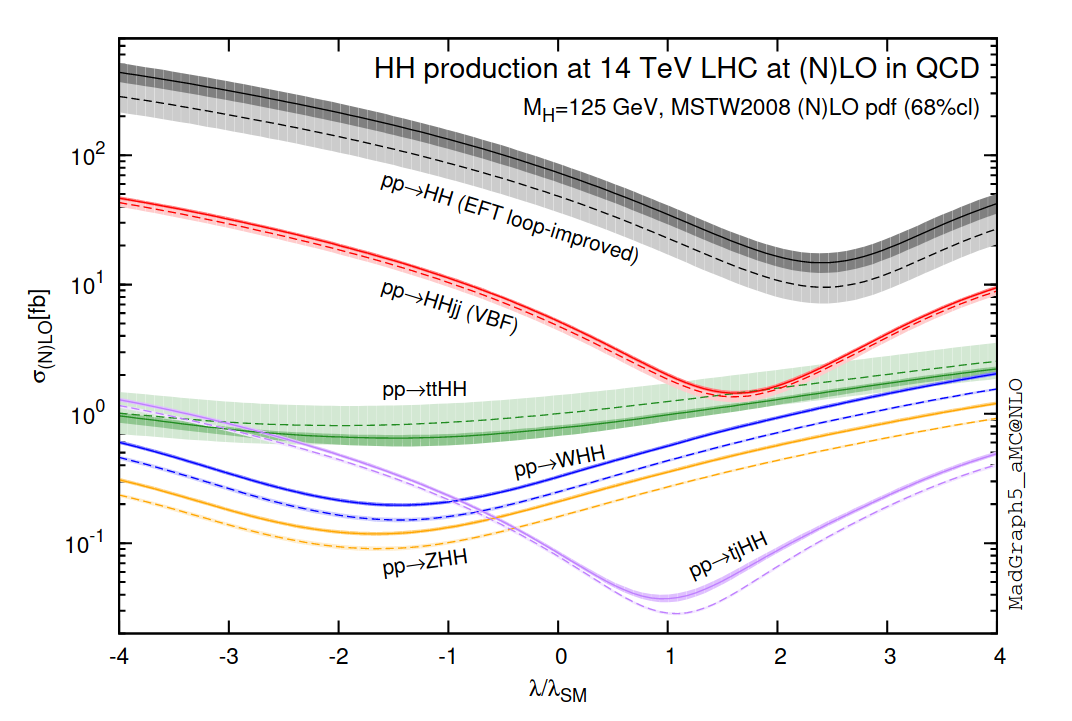
\includegraphics[width=0.7\textwidth]{Part1/Img/HH_Xsec_as_lambda.png}}
\end{figure}

\begin{figure}
    \centering
    \fcolorbox{HHturquoise_m}{HHwhite2}{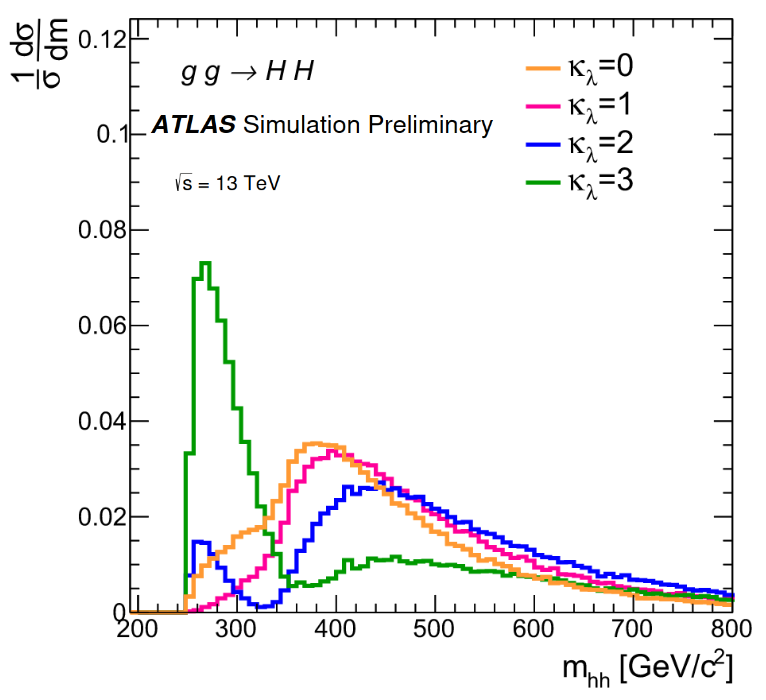
\includegraphics[width=0.7\textwidth]{Part1/Img/mHH.png}}
\end{figure}

\end{columns}
\end{frame}

\begin{frame}{Di-Higgs boson decay modes}

\begin{itemize}
    \item Decay modes of the two Higgs bosons
\end{itemize}
\begin{figure}
    \centering
    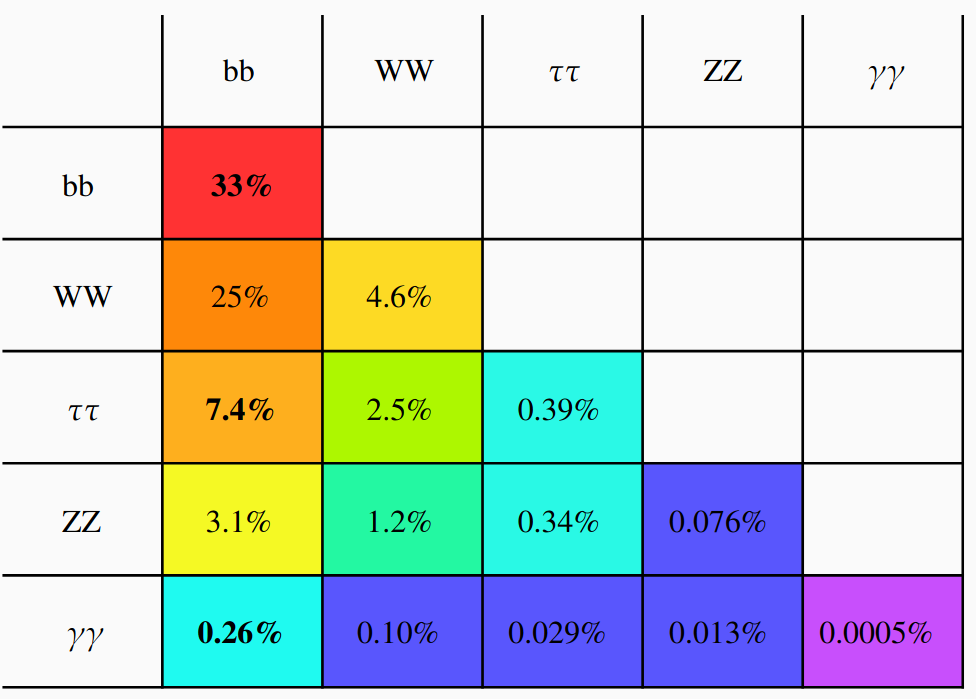
\includegraphics[width=0.43\textwidth]{Part1/Img/HH_decays2.png}
\end{figure}
\pause
\begin{itemize}
    \item \textbf{\textcolor{HHred}{Focusing on HH$\to b\bar{b}\gamma\gamma$} (Golden channel)}
    \item Despite low decay rate, one of the most sensitive channels:
    \begin{itemize}
        \item \textbf{High} H$\to b\bar{b}$ branching ratio
        \item Very \textbf{clean} signature
        \item \textbf{Excellent} $m_{\gamma\gamma}$ mass resolution
        \item \textbf{Good signal extraction}
    \end{itemize}
\end{itemize}

\end{frame}